\section{INSAT-3D Imager SRFs}
%=============================
\label{app.imgr_srf_data_plots}

\subsection{Channel 3}
\begin{figure}[H]
  \label{fig:imgr_ch3}
  \centering
  \begin{tabular}{c}
    \includegraphics[scale=0.55]{graphics/imgr/srf/imgr_insat3d-3.eps} \\
    \includegraphics[scale=0.55]{graphics/imgr/srf/imgr_insat3d-3.difference.eps}
  \end{tabular}
  \caption{INSAT-3D Imager channel 3 spectral responses. Vertical dashed lines are the locations of the computed central frequencies. \emph{(Top)} Comparison of original and new SRFs. \emph{(Bottom)} Response difference between the original and new SRFs.}
\end{figure}

\subsection{Channel 4}
\begin{figure}[H]
  \label{fig:imgr_ch4}
  \centering
  \begin{tabular}{c}
    \includegraphics[scale=0.55]{graphics/imgr/srf/imgr_insat3d-4.eps} \\
    \includegraphics[scale=0.55]{graphics/imgr/srf/imgr_insat3d-4.difference.eps}
  \end{tabular}
  \caption{INSAT-3D Imager channel 4 spectral responses. Vertical dashed lines are the locations of the computed central frequencies. \emph{(Top)} Comparison of original and new SRFs. \emph{(Bottom)} Response difference between the original and new SRFs.}
\end{figure}

\subsection{Channel 5}
\begin{figure}[H]
  \label{fig:imgr_ch5}
  \centering
  \begin{tabular}{c}
    \includegraphics[scale=0.55]{graphics/imgr/srf/imgr_insat3d-5.eps} \\
    \includegraphics[scale=0.55]{graphics/imgr/srf/imgr_insat3d-5.difference.eps}
  \end{tabular}
  \caption{INSAT-3D Imager channel 5 spectral responses. Vertical dashed lines are the locations of the computed central frequencies. \emph{(Top)} Comparison of original and new SRFs. \emph{(Bottom)} Response difference between the original and new SRFs.}
\end{figure}

\subsection{Channel 6}
\begin{figure}[H]
  \label{fig:imgr_ch6}
  \centering
  \begin{tabular}{c}
    \includegraphics[scale=0.55]{graphics/imgr/srf/imgr_insat3d-6.eps} \\
    \includegraphics[scale=0.55]{graphics/imgr/srf/imgr_insat3d-6.difference.eps}
  \end{tabular}
  \caption{INSAT-3D Imager channel 6 spectral responses. Vertical dashed lines are the locations of the computed central frequencies. \emph{(Top)} Comparison of original and new SRFs. \emph{(Bottom)} Response difference between the original and new SRFs.}
\end{figure}
